% Kruskal's algorithm (generated by figs_c1ch10.py).
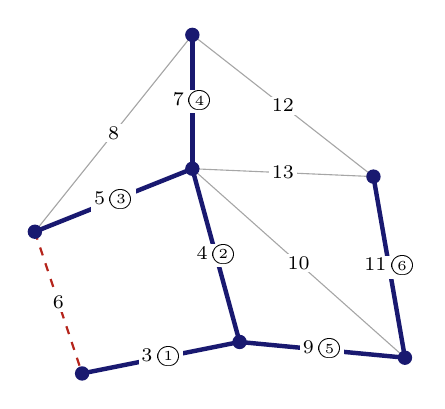
\begin{tikzpicture}[x=1cm,y=1cm,l/.style={font=\footnotesize},c/.style={font=\scriptsize,fill=white,inner sep=1pt}]
\draw[MidnightBlue,line width=1.6pt] (0.6,-1.8) -- (2.6,-1.4);
\node[c] at (1.600,-1.600) {$3$\,\textcircled{\tiny 1}};
\draw[MidnightBlue,line width=1.6pt] (2.6,-1.4) -- (2,0.8);
\node[c] at (2.300,-0.300) {$4$\,\textcircled{\tiny 2}};
\draw[MidnightBlue,line width=1.6pt] (2,0.8) -- (0,0);
\node[c] at (1.000,0.400) {$5$\,\textcircled{\tiny 3}};
\draw[BrickRed,thick,dashed] (0,0) -- (0.6,-1.8);
\node[c] at (0.300,-0.900) {$6$};
\draw[MidnightBlue,line width=1.6pt] (2,0.8) -- (2.0,2.5);
\node[c] at (2.000,1.650) {$7$\,\textcircled{\tiny 4}};
\draw[black!35] (0,0) -- (2.0,2.5);
\node[c] at (1.000,1.250) {$8$};
\draw[MidnightBlue,line width=1.6pt] (2.6,-1.4) -- (4.7,-1.6);
\node[c] at (3.650,-1.500) {$9$\,\textcircled{\tiny 5}};
\draw[black!35] (2,0.8) -- (4.7,-1.6);
\node[c] at (3.350,-0.400) {$10$};
\draw[MidnightBlue,line width=1.6pt] (4.3,0.7) -- (4.7,-1.6);
\node[c] at (4.500,-0.450) {$11$\,\textcircled{\tiny 6}};
\draw[black!35] (2.0,2.5) -- (4.3,0.7);
\node[c] at (3.150,1.600) {$12$};
\draw[black!35] (2,0.8) -- (4.3,0.7);
\node[c] at (3.150,0.750) {$13$};
\fill[MidnightBlue] (0,0) circle (2.6pt);
\fill[MidnightBlue] (2,0.8) circle (2.6pt);
\fill[MidnightBlue] (4.3,0.7) circle (2.6pt);
\fill[MidnightBlue] (0.6,-1.8) circle (2.6pt);
\fill[MidnightBlue] (2.6,-1.4) circle (2.6pt);
\fill[MidnightBlue] (4.7,-1.6) circle (2.6pt);
\fill[MidnightBlue] (2.0,2.5) circle (2.6pt);
\end{tikzpicture}
